\subsection{ERROR REDUCTION}

In this section, we discuss error of analysis of images. The target can be differents forms. However, 
ROI is rectangular window. We identify certains areas inside of ROI that has more importance than others.
In Fig. \ref{fig:erroridentified}, there are an error points close of edges because target not occupies whole ROI. 

\begin{figure}[H]
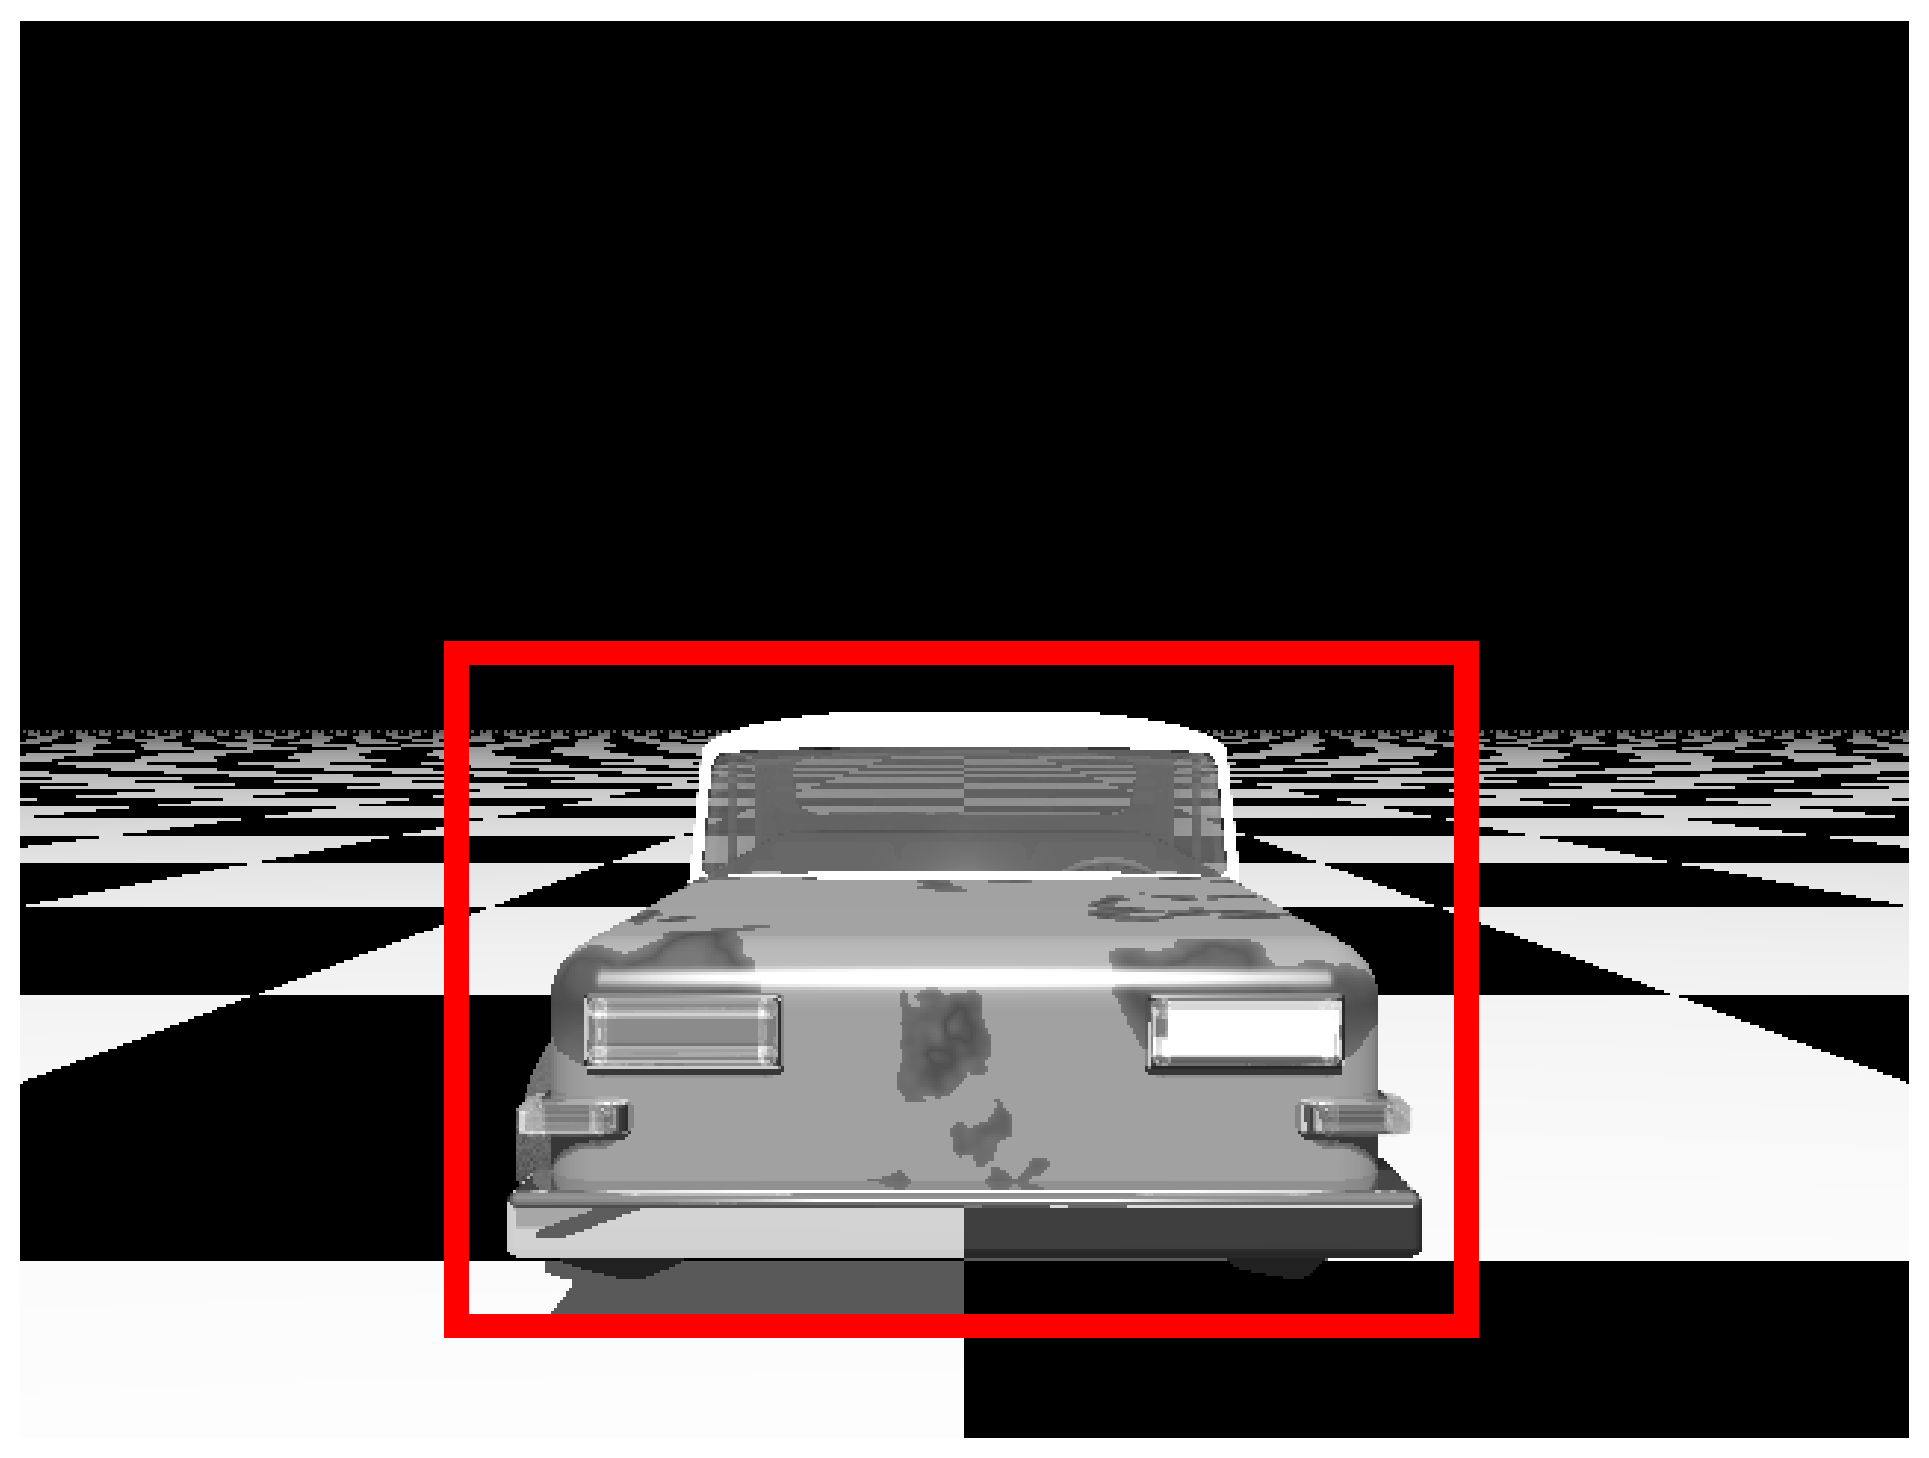
\includegraphics[width=\columnwidth]{images/imageError.eps}
\caption{Illustration of ROI with error close at edges}
\label{fig:erroridentified}
\end{figure}

The rectangular window is used to correlation. In PCC, two matrix at same dimensios can be compared. 
It's not possible for this correlation generate any date with imagens of differents dimensions. 
However, PCC has high precision in its analysis.

We decide solve this problem given a ponderation in PCC. Then, Points that contained the target was considered plus important
and points of less importance has low weight in correlation.

\begin{figure}[H]
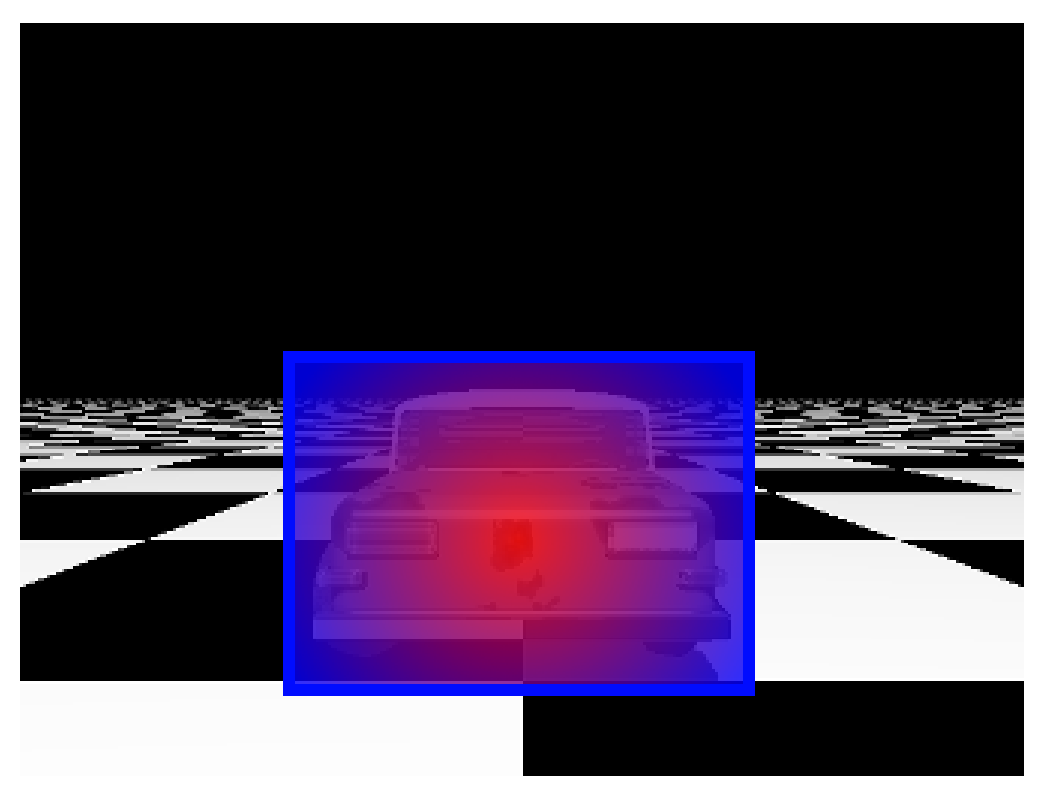
\includegraphics[width=\columnwidth]{images/imageErrorcontroled.eps}
\caption{Illustration of points of most importance (red) and points less importance (blue) in correlation.}
\label{fig:errorpondered}
\end{figure}

Points close of edge have less importance and they are in blue in Fig. \ref{fig:errorpondered}. 
Points close of center of image are red and, probably, they is on the object.